\section{Benchmark NIST-8 "Oscillatory"}
\label{sec:bench-8}

This is a wave function that satisfies the Schrodinger's equation model of two
interacting atoms, highly oscillatory near the origin.
The equation solved is

\begin{equation} \label{oscillatory}
-\nabla^{2} u - \frac{1}{(\alpha + r)^{4}} u = f,
\end{equation}
in the domain $\Omega = (0, 1)^2$, equipped with Dirichlet boundary conditions
given by the exact solution.

The exact solution:
\begin{equation}\label{exact-nist-8}
u(x,y) = sin(\frac{1}{\alpha + r}),
\end{equation}
where $r = \sqrt{x^{2} + y^{2}}$, $\alpha = \frac{1}{N \pi}$ determines the number of oscillations.
The right-hand side $f$ is calculated by inserting (\ref{exact-nist-8}) into (\ref{oscillatory}).
The solution of NIST-8 with $\alpha = \frac{1}{10 \pi}$ is shown in Fig. \ref{fig:sln-nist08}.

\begin{figure}[!ht]
\centering
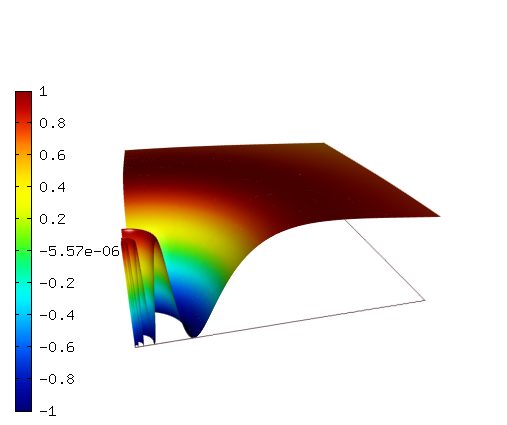
\includegraphics[height=6cm]{nist/nist-8/solution.png}
\caption{The solution to NIST-8 benchmark problem.}
\label{fig:sln-nist08}
\end{figure}
